\documentclass[a4paper]{article}

\usepackage[T1]{fontenc}
\usepackage[utf8]{inputenc}
\usepackage{lmodern}

\newcommand{\ttsl}[1]{\texttt{\textsl{#1}}}
\usepackage{pgf-soroban}

\title{SOROBAN abacus\\\ \\package \texttt{pgf-soroban}}
\author{Alain Delmotte \texttt{esperanto@swing.be}}
\date{November 27, 2013}

\begin{document}
\maketitle
\tableofcontents
\newpage

\section{Original size} 

\begin{center}
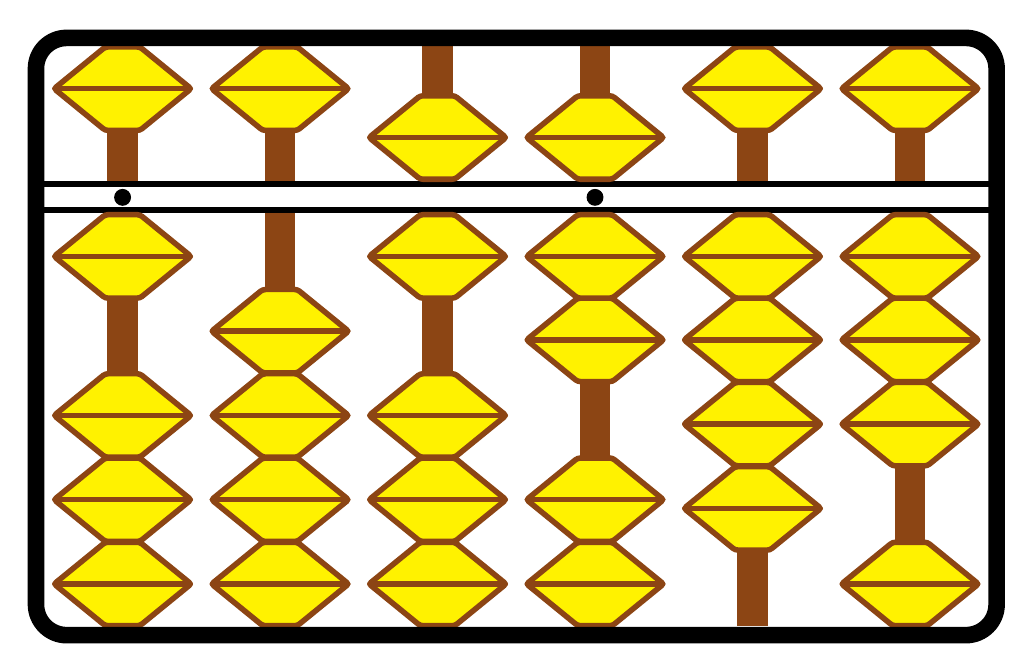
\begin{tikzpicture}
\tige{1}{1}{1}
\tige{2}{0}{0}
\tige{3}{6}{0}
\tige{4}{7}{1}
\tige{5}{4}{0}
\tige{6}{3}{0}
\cadre{6}
\end{tikzpicture}
\end{center}
\vspace{10mm}

\section{Example of use}

\textbf{Step 1}
\vspace{10mm}
\ladj{0.25}
\textbf{2 + 1} (in colours)\\
1) Put 2 with thumb
\hspace*{5mm}
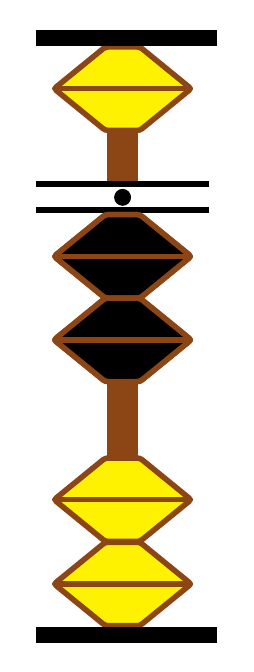
\begin{tikzpicture}
\tige{1}{2}{1}
\binoire{1}{5}{black}
\binoire{1}{6}{black}
\barres{1}
\end{tikzpicture}
\quad 2) Add 1
\hspace*{5mm}
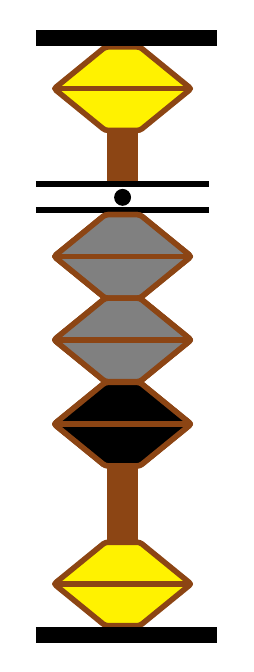
\begin{tikzpicture}
\tige{1}{3}{1}
\binoire{1}{5}{gray}
\binoire{1}{6}{gray}
\binoire{1}{7}{black}
\barres{1}
\end{tikzpicture}
\quad 
\hspace{5mm}$\Rightarrow$ \textbf{= 3}\hspace{5mm}
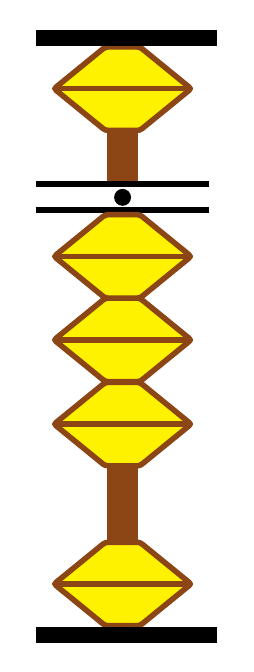
\begin{tikzpicture}
\tige{1}{3}{1}
\barres{1}
\end{tikzpicture}
\vspace{15mm}

\renewcommand{\colbil}{white}
\renewcommand{\coltig}{darkgray}
\noindent\textbf{7 - 1} (in black and white for printing)\\
1) Set 7 at once (pinch)\hspace*{5mm}
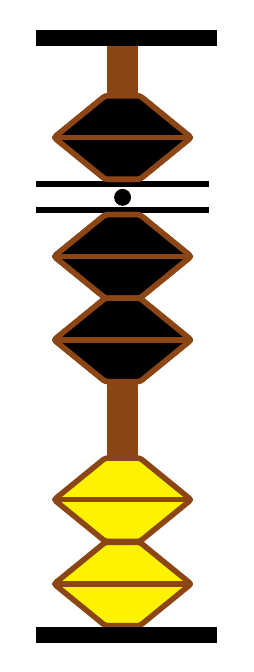
\begin{tikzpicture}
\tige{1}{7}{1}
\binoire{1}{5}{black}
\binoire{1}{6}{black}
\binoire{1}{10}{black}
\barres{1}
\end{tikzpicture}
\quad 2) Substract 1
\hspace*{5mm}
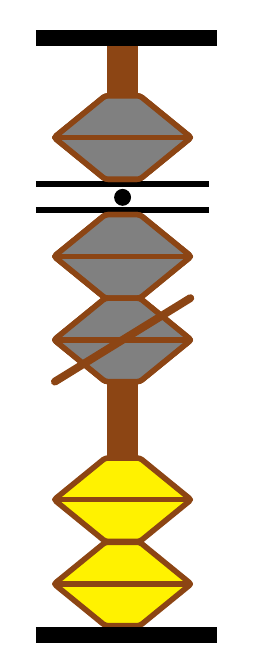
\begin{tikzpicture}
\tige{1}{7}{1}
\binoire{1}{5}{gray}
\binoire{1}{6}{gray}
\binoire{1}{10}{gray}
\barbil{1}{6}
\barres{1}
\end{tikzpicture}
\quad 
\hspace{5mm}$\Rightarrow$ \textbf{= 6}\hspace{5mm}
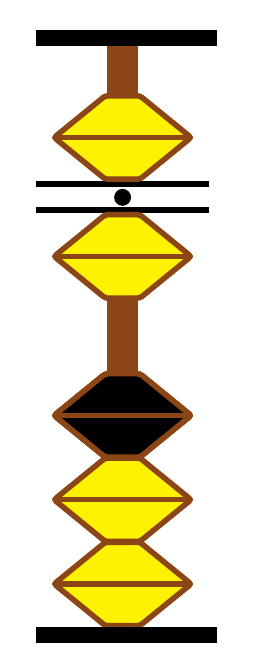
\begin{tikzpicture}
\tige{1}{6}{1}
\binoire{1}{3}{black}
\barres{1}
\end{tikzpicture}
\newpage

\section{Using the package}

In the preamble, insert the instruction \verb+\usepackage{pgf-soroban}+~\footnote{\ There is a corresponding package \texttt{pst-soroban.sty} for use with Pstricks.}. There is
no need to load the corresponding graphics package as the packages are required
by the soroban package.

The package also sets a base unit as 1 mm, as well as other lengths; this draws a soroban of the normal size as used in schools, shops,\dots If one wants to change the size, one sets the units by \verb+\ladj{0.25}+ (here $\frac 14$ of the normal size). That instruction can be used any time in the document to change the size for some part if required.

To draw a soroban, one draws rod(s) with the required bids in the right position and add either a frame or just top and bottom parts of the frame. One can then add some bids in other colours and also cross some bids.

Let's draw a soroban representing the number 321.45 in small size: 0.25.

\renewcommand{\colbil}{yellow}
\renewcommand{\coltig}{brun}
\ladj{0.25}
\begin{center}
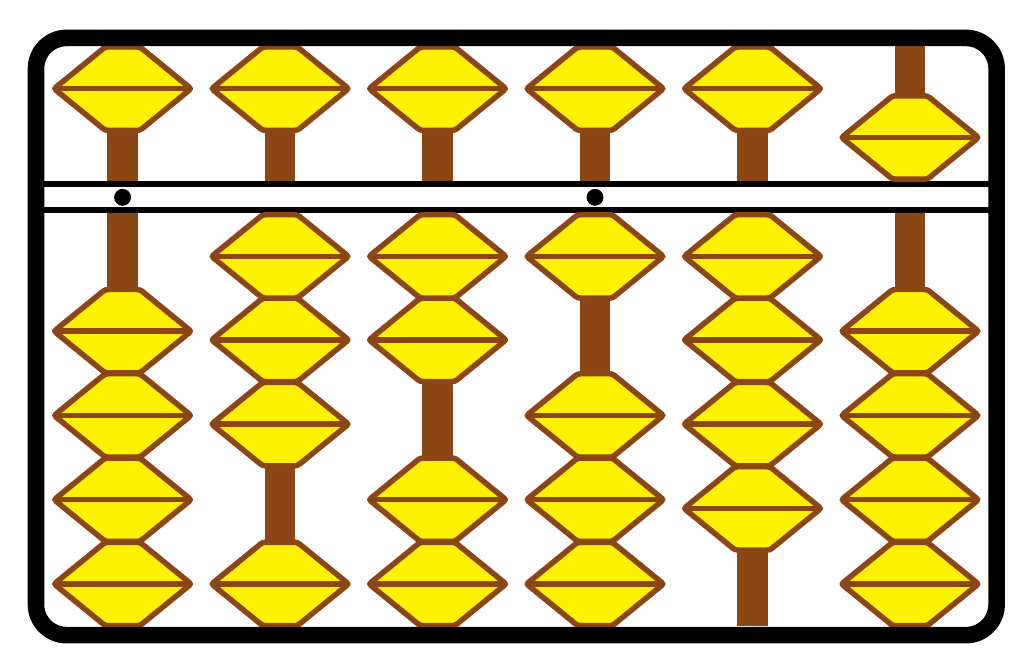
\begin{tikzpicture}
\tige{1}{0}{1}
\tige{2}{3}{0}
\tige{3}{2}{0}
\tige{4}{1}{1}
\tige{5}{4}{0}
\tige{6}{5}{0} 
\cadre{6}
\end{tikzpicture}
\end{center}
\begin{tabular}{|l|l|l|}
\hline
\textbf{line}& \textbf{tikz/pgf} & \textbf{PStricks} \\
\hline
\verb| 1| & \verb|\ladj{0.25}|         & \verb|\psset{unit=0.25mm}             |\\
\verb| 2| & \verb|\begin{tikzpicture}| & \verb|\begin{pspicture}(-2,-2)(122,76)|\\
\verb| 3| & \verb|\tige{1}{0}{1}     | & \verb|\tige{1}{0}{1}                  |\\
\verb| 4| & \verb|\tige{2}{3}{0}     | & \verb|\tige{2}{3}{0}                  |\\
\verb| 5| & \verb|\tige{3}{2}{0}     | & \verb|\tige{3}{2}{0}                  |\\
\verb| 6| & \verb|\tige{4}{1}{1}     | & \verb|\tige{4}{1}{1}                  |\\
\verb| 7| & \verb|\tige{5}{4}{0}     | & \verb|\tige{5}{4}{0}                  |\\
\verb| 8| & \verb|\tige{6}{5}{0}     | & \verb|\tige{6}{5}{0}                  |\\
\verb| 9| & \verb|\cadre{6}          | & \verb|\cadre{6}                       |\\
\verb|10| & \verb|\end{tikzpicture}  | & \verb|\end{pspicture}                 |\\
\hline
\end{tabular}
\vspace{6pt}

Line 1 defines the size, lines 2 and 10 create the picture environment, lines 3--8 draw the rods and line 9 creates the frame. Lines 3 and 6 specify a dotted rod (third argument = 1), the values (0, 3, 2, 1, 4 and 5) are in the second argument

It is not necessary for tikz to specify the dimensions of the picture as the package reserves the area needed for the created graphic.~\footnote{\ For PStricks (\texttt{pst-soroban}), one has to give the dimensions of the picture, otherwise the drawing would have no size and would overlap the surrounding text. One gives some space before and below (\texttt{(-2,-2)}) and after above. The picture is 74.6 units hight and 20* number of rods wide (here \texttt{(122,76)}). Of course, if one adds something before, under, after or above the soroban, one has to adjust the corresponding part of the frame dimension.}

To draw a rod, one uses the command \verb+\tige+. The syntax is:
\begin{center}
\verb|\tige[|\ttsl{<st>}\verb|]{|\ttsl{<nu>}\verb|}{|\ttsl{<val>}\verb|}{|\ttsl{<un>}\verb|}|
\end{center}

The \ttsl{<nu>} argument numbers the rods from left to right. \ttsl{<val>} is the number to be represented on the rod from 0 to 9. The \ttsl{<un>} argument tells that there is a dot on the central bar (1) or not (0); there is normally a dot for the unit, thousand, million,\dots ranks.

The \ttsl{<st>} argument is optional and tells at which position the drawing is started; the default value is 1. This is interesting when one wants to put more then one drawing on a line:

\begin{center}
\begin{minipage}[][][c]{5cm}
\begin{verbatim}
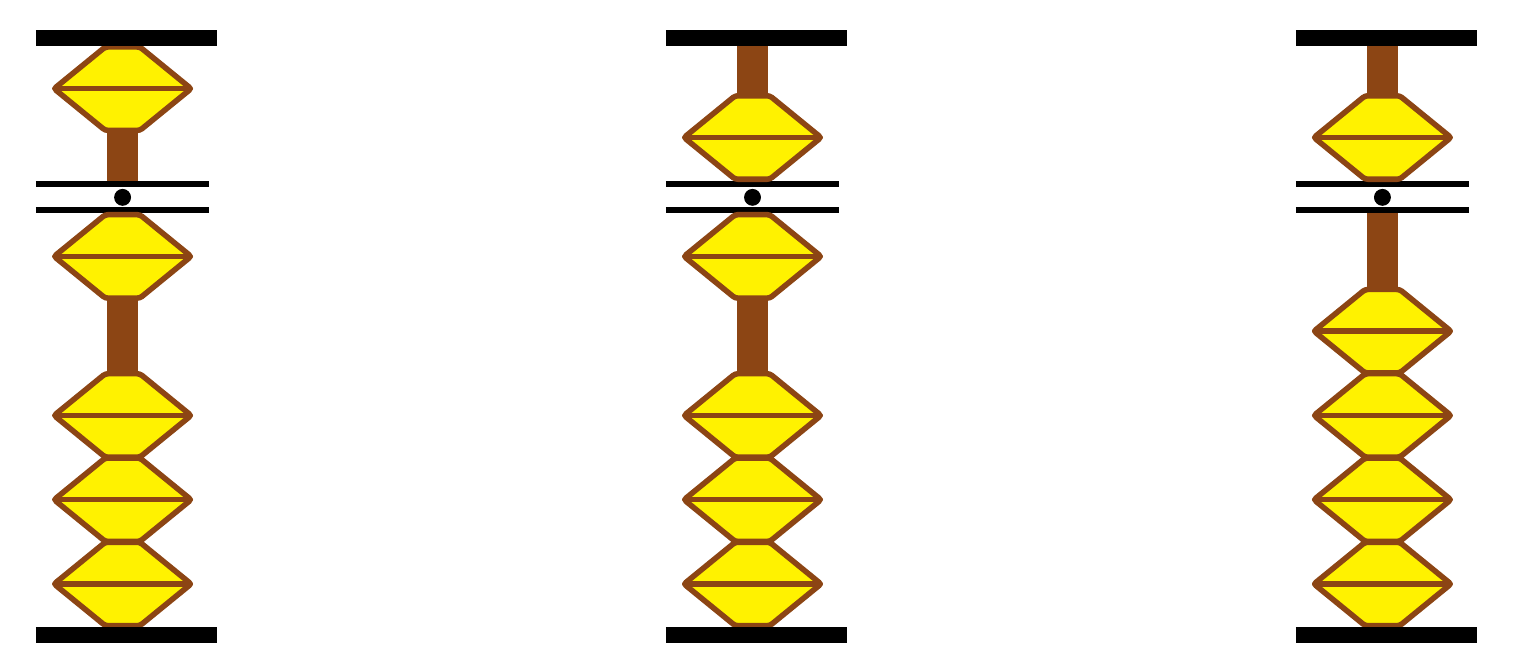
\begin{tikzpicture}
\tige{1}{1}{1}
\barres{1}
\tige[5]{1}{6}{1}
\barres[5]{1}
\tige[9]{1}{5}{1}
\barres[9]{1}
\end{tikzpicture}
\end{verbatim}
\end{minipage}
\hspace{10mm}
\begin{minipage}[][][c]{5cm}
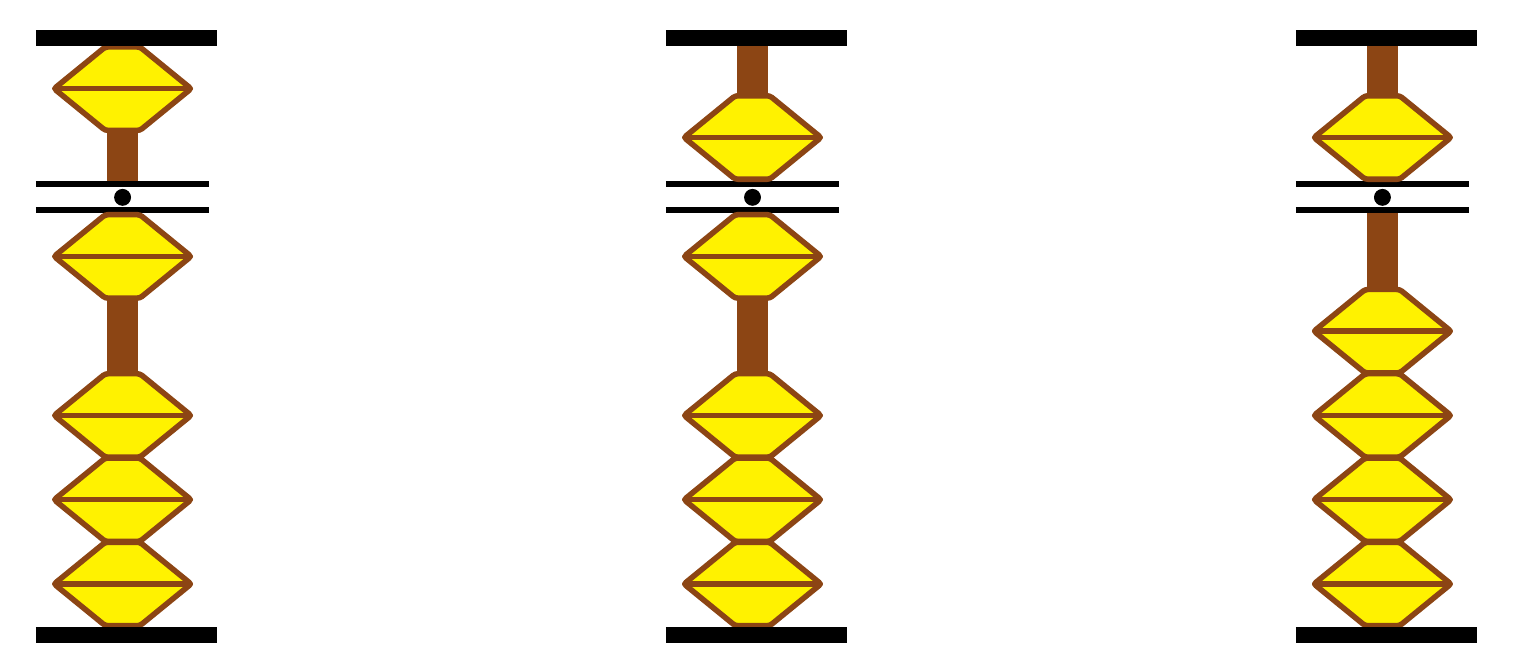
\begin{tikzpicture}
\tige{1}{1}{1}
\barres{1}
\tige[5]{1}{6}{1}
\barres[5]{1}
\tige[9]{1}{5}{1}
\barres[9]{1}
\end{tikzpicture}
\end{minipage}
\end{center}

In this example, there is no frame but only parts of it above and below; this is created with the \verb+\barres+ command. The syntaxes for the frame and top/bottom lines are:
\begin{center}
\verb|\cadre[|\ttsl{<st>}\verb|]{|\ttsl{<nb>}\verb|}| and \verb|\barres[|\ttsl{<st>}\verb|]{|\ttsl{<nb>}\verb|}|.
\end{center}

The optional \ttsl{<st>} arguments are the same as the one of \verb+\tige+, the \ttsl{<nb>} argument tell how many rods have to be covered.

If one wants to colour a specific bid , one can achieve this with \verb+\binoire+:
\begin{center}
\verb|\binoire[|\ttsl{<st>}\verb|]{|\ttsl{<nu>}\verb|}{|\ttsl{<pos>}\verb|}{|\ttsl{<col>}\verb|}|
\end{center}

\ttsl{<st>} and \ttsl{<nu>} arguments are the same as for \verb+\tige+; the \ttsl{<col>} argument defines the colour and the \ttsl{<pos>} argument tells which bid has to be coloured as shown in the following example.

\begin{center}
\begin{minipage}[c]{5cm}
\begin{verbatim}
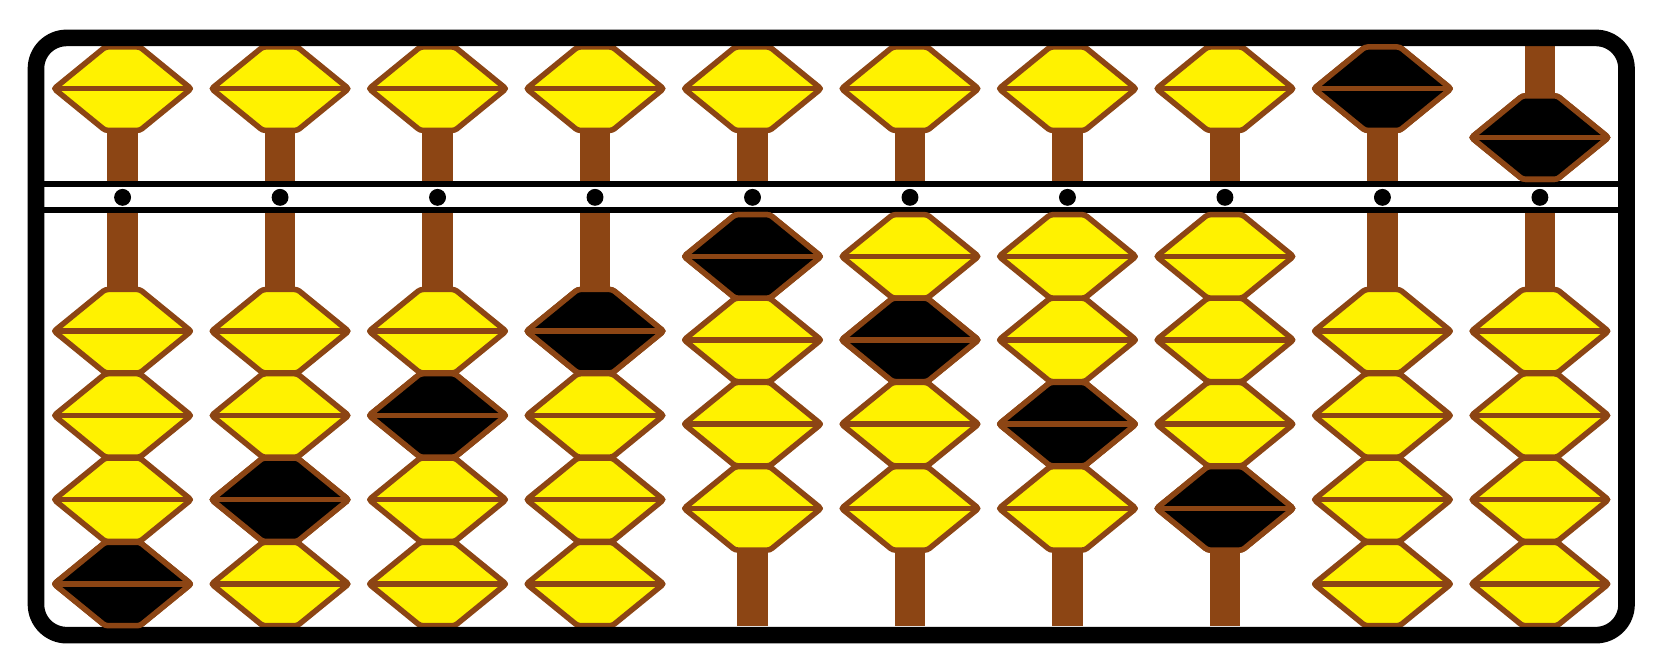
\begin{tikzpicture}
\tige{1}{0}{1}
\tige{2}{0}{1}
\tige{3}{0}{1}
\tige{4}{0}{1}
\tige{5}{4}{1}
\tige{6}{4}{1}
\tige{7}{4}{1}
\tige{8}{4}{1}
\tige{9}{0}{1}
\tige{10}{5}{1}
\cadre{10}
\binoire{1}{1}{black}
\binoire{2}{2}{black}
\binoire{3}{3}{black}
\binoire{4}{4}{black}
\binoire{5}{5}{black}
\binoire{6}{6}{black}
\binoire{7}{7}{black}
\binoire{8}{8}{black}
\binoire{9}{9}{black}
\binoire{10}{10}{black}
\end{tikzpicture}
\end{verbatim}
\end{minipage}
\hspace{10mm}
\begin{minipage}[][][c]{5cm}
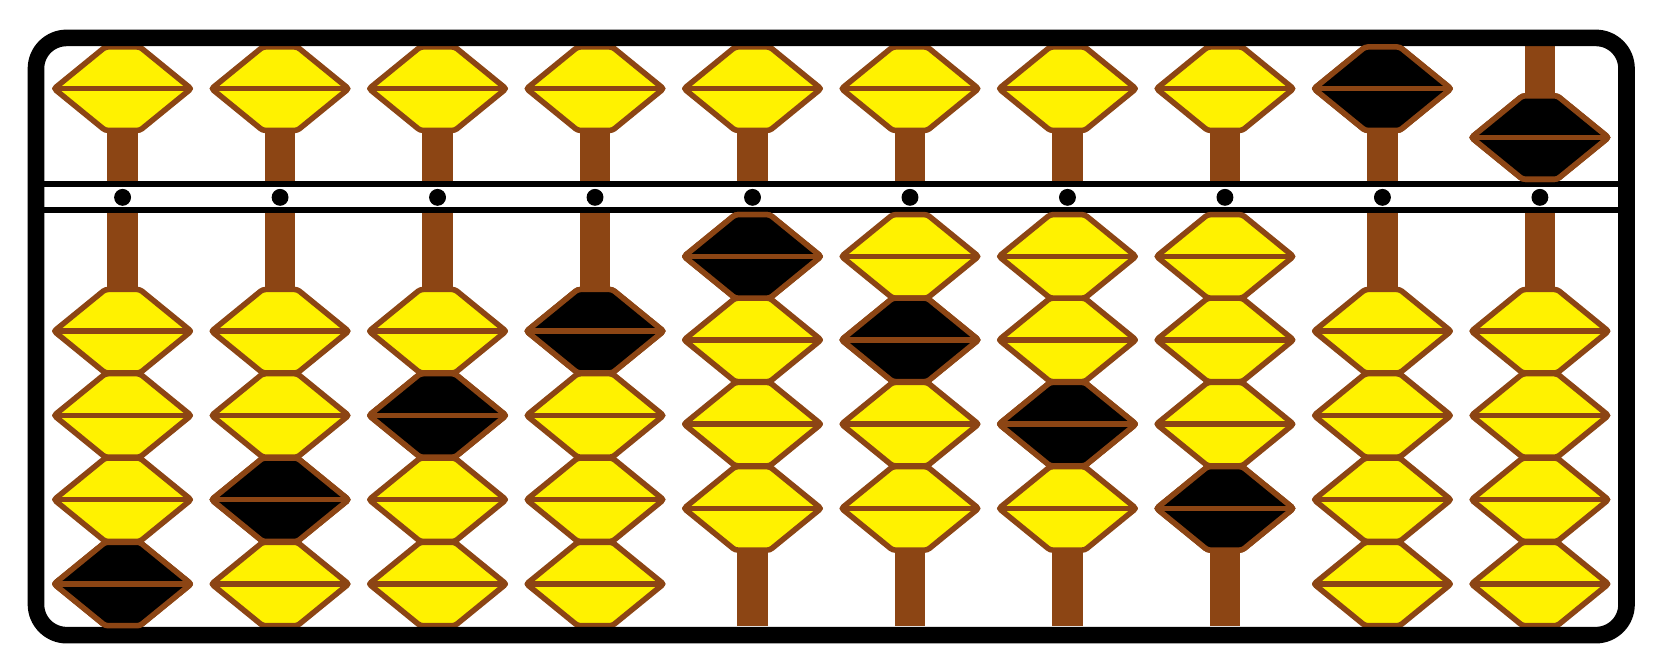
\begin{tikzpicture}
\tige{1}{0}{1}
\tige{2}{0}{1}
\tige{3}{0}{1}
\tige{4}{0}{1}
\tige{5}{4}{1}
\tige{6}{4}{1}
\tige{7}{4}{1}
\tige{8}{4}{1}
\tige{9}{0}{1}
\tige{10}{5}{1}
\cadre{10}
\binoire{1}{1}{black}
\binoire{2}{2}{black}
\binoire{3}{3}{black}
\binoire{4}{4}{black}
\binoire{5}{5}{black}
\binoire{6}{6}{black}
\binoire{7}{7}{black}
\binoire{8}{8}{black}
\binoire{9}{9}{black}
\binoire{10}{10}{black}
\end{tikzpicture}
\end{minipage}
\end{center}

The \verb+\barbil+ command allows to cross a bid (see example below); the syntax is:
\begin{center}
\verb|\barbil[|\ttsl{<st>}\verb|]{|\ttsl{<nu>}\verb|}{|\ttsl{<pos>}\verb|}|
\end{center}
The arguments \ttsl{<st>}, \ttsl{<nu>} and \ttsl{<pos>} have the same meaning as those of \verb+\binoire+.

Finally, one can change the overall colours of the rods and the bids, for example to print in black and white.
This is done by changing the values of the \verb+\colbil+ (for the bids) and \verb+\coltig+ (for the rods) commands; by default there are ``yellow'' and ``brun'' (new brown colour defined in the package).

\begin{center}
\begin{minipage}[][][c]{5cm}
\begin{verbatim}
\renewcommand{\colbil}{white}
\renewcommand{\coltig}{black}
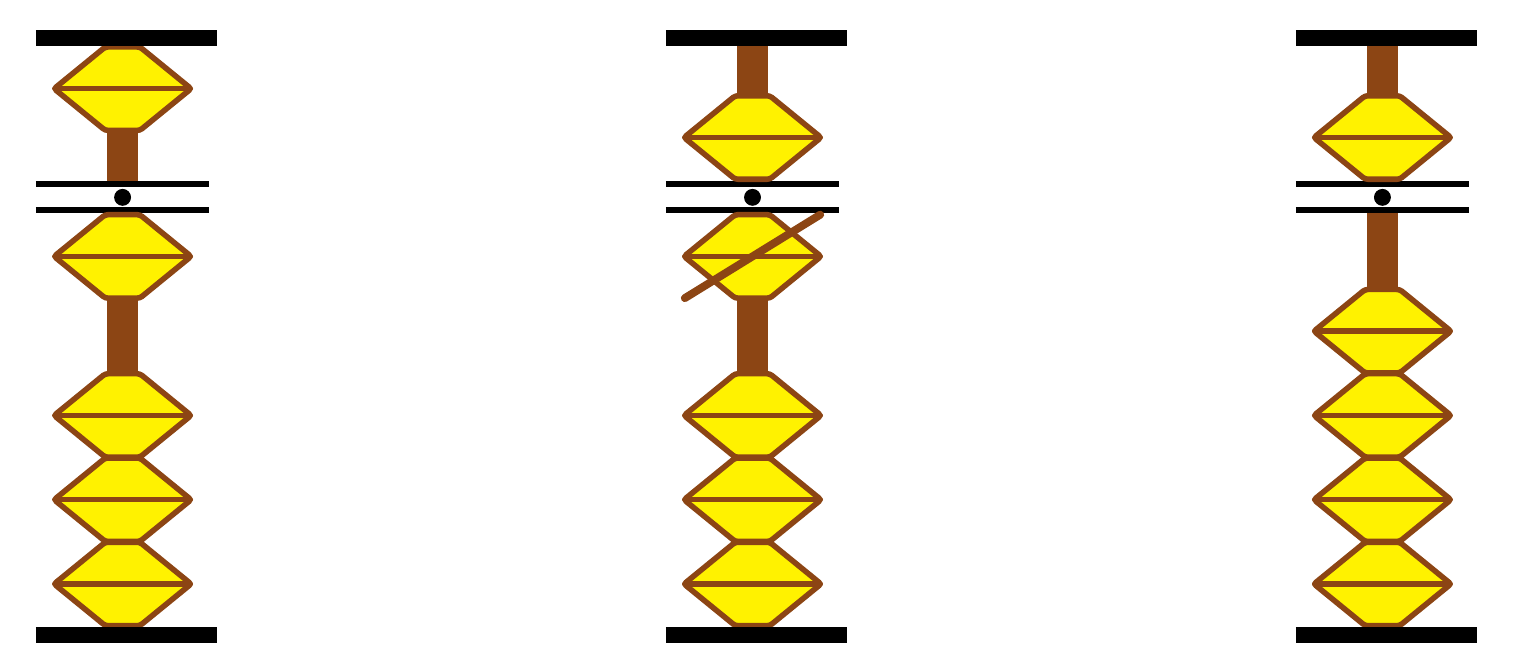
\begin{tikzpicture}
\tige{1}{1}{1}
\barres{1}
\tige[5]{1}{6}{1}
\barbil[5]{1}{5}
\barres[5]{1}
\tige[9]{1}{5}{1}
\barres[9]{1}
\end{tikzpicture}
\end{verbatim}
\end{minipage}
\hspace{10mm}
\renewcommand{\colbil}{white}
\renewcommand{\coltig}{black}
\begin{minipage}[][][c]{5cm}
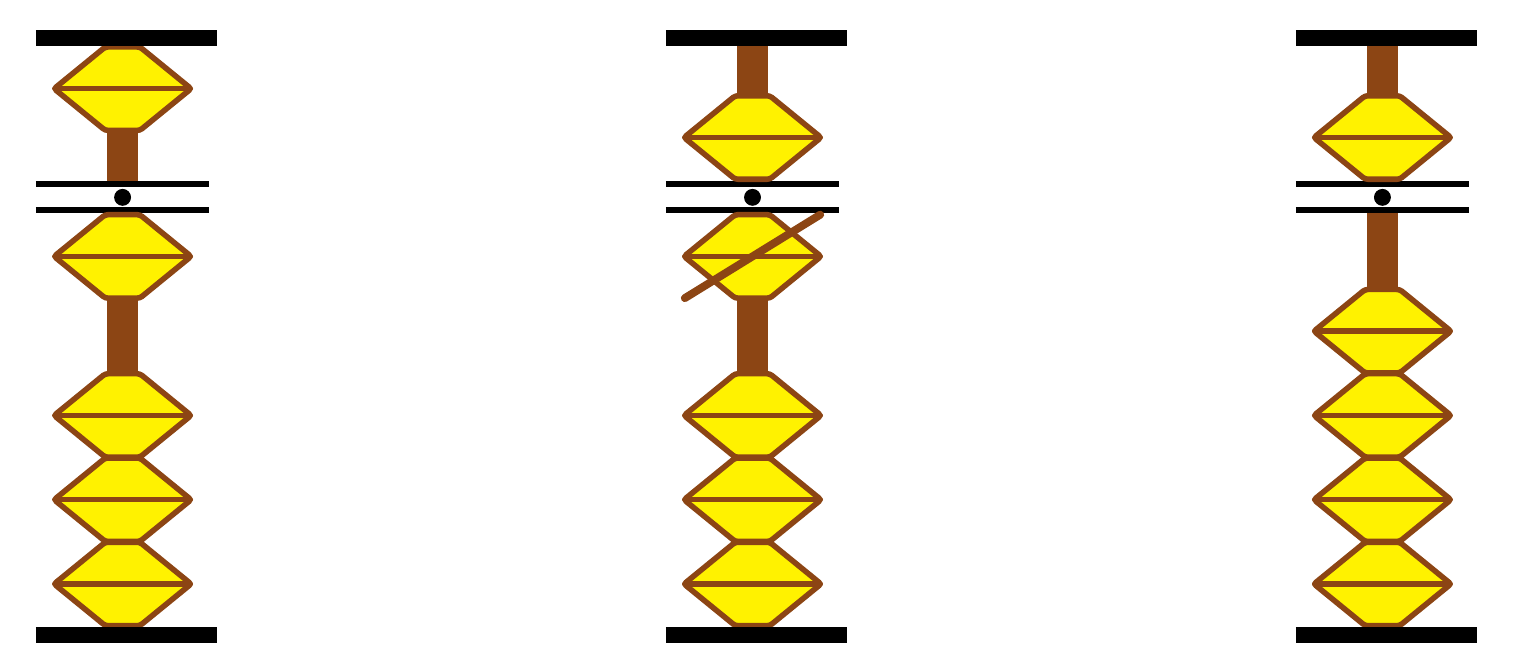
\begin{tikzpicture}
\tige{1}{1}{1}
\barres{1}
\tige[5]{1}{6}{1}
\barbil[5]{1}{5}
\barres[5]{1}
\tige[9]{1}{5}{1}
\barres[9]{1}
\end{tikzpicture}
\end{minipage}
\end{center}

\nocite{*}
\bgroup
\raggedright
\bibliographystyle{plain}
\bibliography{\jobname}
\egroup

\end{document}


